\documentclass[DIN, pagenumber=false, fontsize=11pt, parskip=half]{scrartcl}

\usepackage{amsmath}
\usepackage{amsfonts}
\usepackage{amssymb}
\usepackage{enumitem}
\usepackage[utf8]{inputenc} 
\usepackage[ngerman]{babel} 
\usepackage[T1]{fontenc} 
\usepackage{pgfplots}
\usepackage{xcolor}
\usepackage{listings}
\usepackage{float}
\usepackage{graphicx}
\usepackage{booktabs}
\usepackage{tkz-euclide}

\definecolor{mygreen}{RGB}{28,172,0} % color values Red, Green, Blue
\definecolor{mylilas}{RGB}{170,55,241}

\tikzstyle{neuron}=[circle,fill=black!25,minimum size=30pt,inner sep=0pt]

\lstset{language=Matlab,%
    %basicstyle=\color{red},
    breaklines=true,%
    morekeywords={matlab2tikz},
    keywordstyle=\color{blue},%
    morekeywords=[2]{1}, keywordstyle=[2]{\color{black}},
    identifierstyle=\color{black},%
    stringstyle=\color{mylilas},
    commentstyle=\color{mygreen},%
    showstringspaces=false,%without this there will be a symbol in the places where there is a space
    numbers=left,%
    numberstyle={\tiny \color{black}},% size of the numbers
    numbersep=9pt, % this defines how far the numbers are from the text
    emph=[1]{for,end,break},emphstyle=[1]\color{red}, %some words to emphasise
    %emph=[2]{word1,word2}, emphstyle=[2]{style},    
}

\title{Einführung in die Neuroinformatik}
\author{Tim Luchterhand, Paul Nykiel (Gruppe P)}

\begin{document}
    \maketitle
    \section{Lernschritt im Perzeptron-Lernalgorithmus}
    \begin{enumerate}[label=(\alph*)]
        \item
            \begin{eqnarray*}
                w_1 \cdot x_1 + w_2 \cdot x_2 + w_0 &=& 0 \\
                \Leftrightarrow x_2 &=& -\frac{w_1 \cdot x_1 + w_0}{w_2} \\
                x_2 &=& -\frac{1}{2} x_1 + \frac{1}{2}
            \end{eqnarray*}
            \begin{figure}[H]
                \centering
                \begin{tikzpicture}
                    \tkzInit[xmax=3,ymax=3,xmin=-3,ymin=-3]
                    \tkzGrid
                    \tkzAxeXY
                    \draw[thick,latex-latex, color=red, ->] (0,0) -- (1,2) node[anchor=south west] {$w$}; 
                    \fill (2,2) circle [radius=0.08];
                    \draw (2,2) node[anchor=south west] {$x$};
                    \draw[thick, color=green] (-3,2) -- (3, -1) node[anchor=south west]{Separierungslinie};
                \end{tikzpicture}
            \end{figure}
        \item
            \begin{eqnarray*}
                w^* &=& \begin{pmatrix}
                    1 \\ 2\\ -1
                \end{pmatrix} \\
                x^* &=& \begin{pmatrix}
                    2 \\ 2\\ 1
                \end{pmatrix}
            \end{eqnarray*}
        \item $w_1$ in \textcolor{red}{rot}, $w_{-1}$ in \textcolor{blue}{blau}
            \begin{figure}[H]
                \centering
                \begin{tikzpicture}
                    \tkzInit[xmax=3,ymax=3,xmin=-3,ymin=-3]
                    \tkzGrid
                    \tkzAxeXY
                    \draw[thick,latex-latex, color=red, ->] (0,0) -- (1,2) node[anchor=south west] {$w$}; 
                    \fill (2,2) circle [radius=0.08];
                    \draw (2,2) node[anchor=south west] {$x$};
                    \draw[thick, color=green] (-3,2) -- (3, -1) node[anchor=south west]{Separierungslinie};
                    \fill[opacity=0.5, color=red] (-3,2) -- (3,-1) -- (3,3) -- (-3,3) -- cycle;
                    \fill[opacity=0.5, color=blue] (-3,2) -- (3,-1) -- (3,-3) -- (-3,-3) -- cycle;
                \end{tikzpicture}
            \end{figure}
        \item Überprüfen ob bereits korrekt klassifiziert:
            \begin{eqnarray*}
                {(w^*)}^T \cdot x^* &=& 2 + 4 - 1 = 5 \geq 0 \\
                &\Rightarrow& x^* \in \omega_{1}
            \end{eqnarray*}
            Lernschritt durchführen:
            \begin{eqnarray*}
                \tilde{w}^* &=& w^* - \eta \cdot x^* = \begin{pmatrix}
                    -1 \\ 0 \\ -2 
                \end{pmatrix} \\
                \Rightarrow \tilde{w} &=& 
                    \begin{pmatrix}
                        -1 \\ 0
                    \end{pmatrix} \\
                \tilde{w}_0 &=& -2
            \end{eqnarray*}
        \item $w_1$ in \textcolor{red}{rot}, $w_{-1}$ in \textcolor{blue}{blau}
            \begin{figure}[H]
                \centering
                \begin{tikzpicture}
                    \tkzInit[xmax=3,ymax=3,xmin=-3,ymin=-3]
                    \tkzGrid
                    \tkzAxeXY
                    \draw[thick,latex-latex, color=red, ->] (0,0) -- (-1,0) node[anchor=south west] {$w$}; 
                    \fill (2,2) circle [radius=0.08];
                    \draw (2,2) node[anchor=south west] {$x$};
                    \draw[thick, color=green] (-2,3) -- (-2, -3) node[anchor=south west]{Separierungslinie};
                    \fill[opacity=0.5, color=blue] (-2,3) -- (-2,-3) -- (3,-3) -- (3,3) -- cycle;
                    \fill[opacity=0.5, color=red] (-2,3) -- (-2,-3) -- (-3,-3) -- (-3,3) -- cycle;
                \end{tikzpicture}
            \end{figure}
        \item Überprüfen ob bereits korrekt klassifiziert:
            \begin{eqnarray*}
                {(\tilde{w}^*)}^T \cdot x^*
                &=& -2 + 0 -2 = -4 \\
                &\Rightarrow& x^* \in \omega_{-1}
            \end{eqnarray*}
            Kein Lernschritt ist notwendig $\Rightarrow w$ wird nicht verändert
    \end{enumerate}
    \section{Perzeptron-Lernalgorithmus}
    Matlab script:
    \lstinputlisting{b04a02.m}
    \begin{figure}[H]
        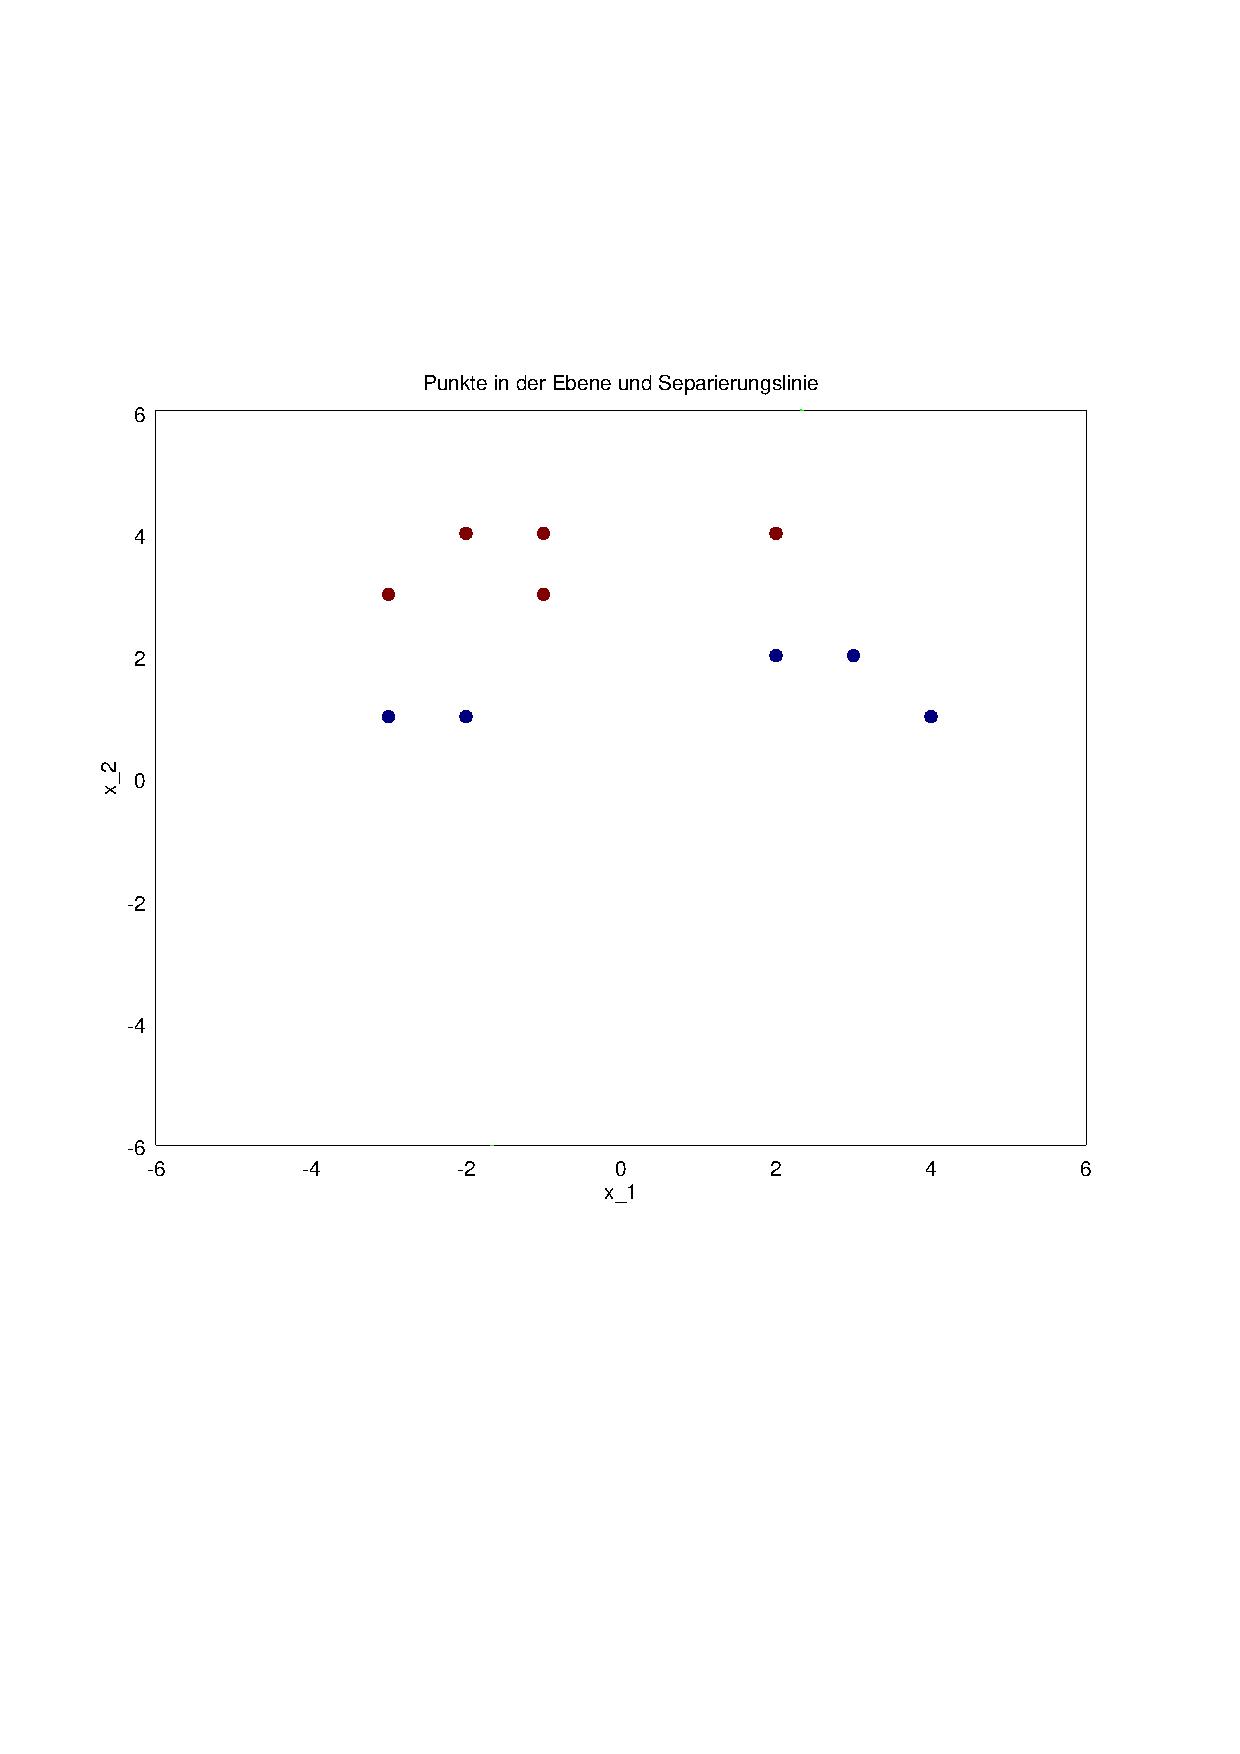
\includegraphics[width=\textwidth]{initial}
        \caption{Anfangszustand}
    \end{figure}
    \begin{figure}[H]
        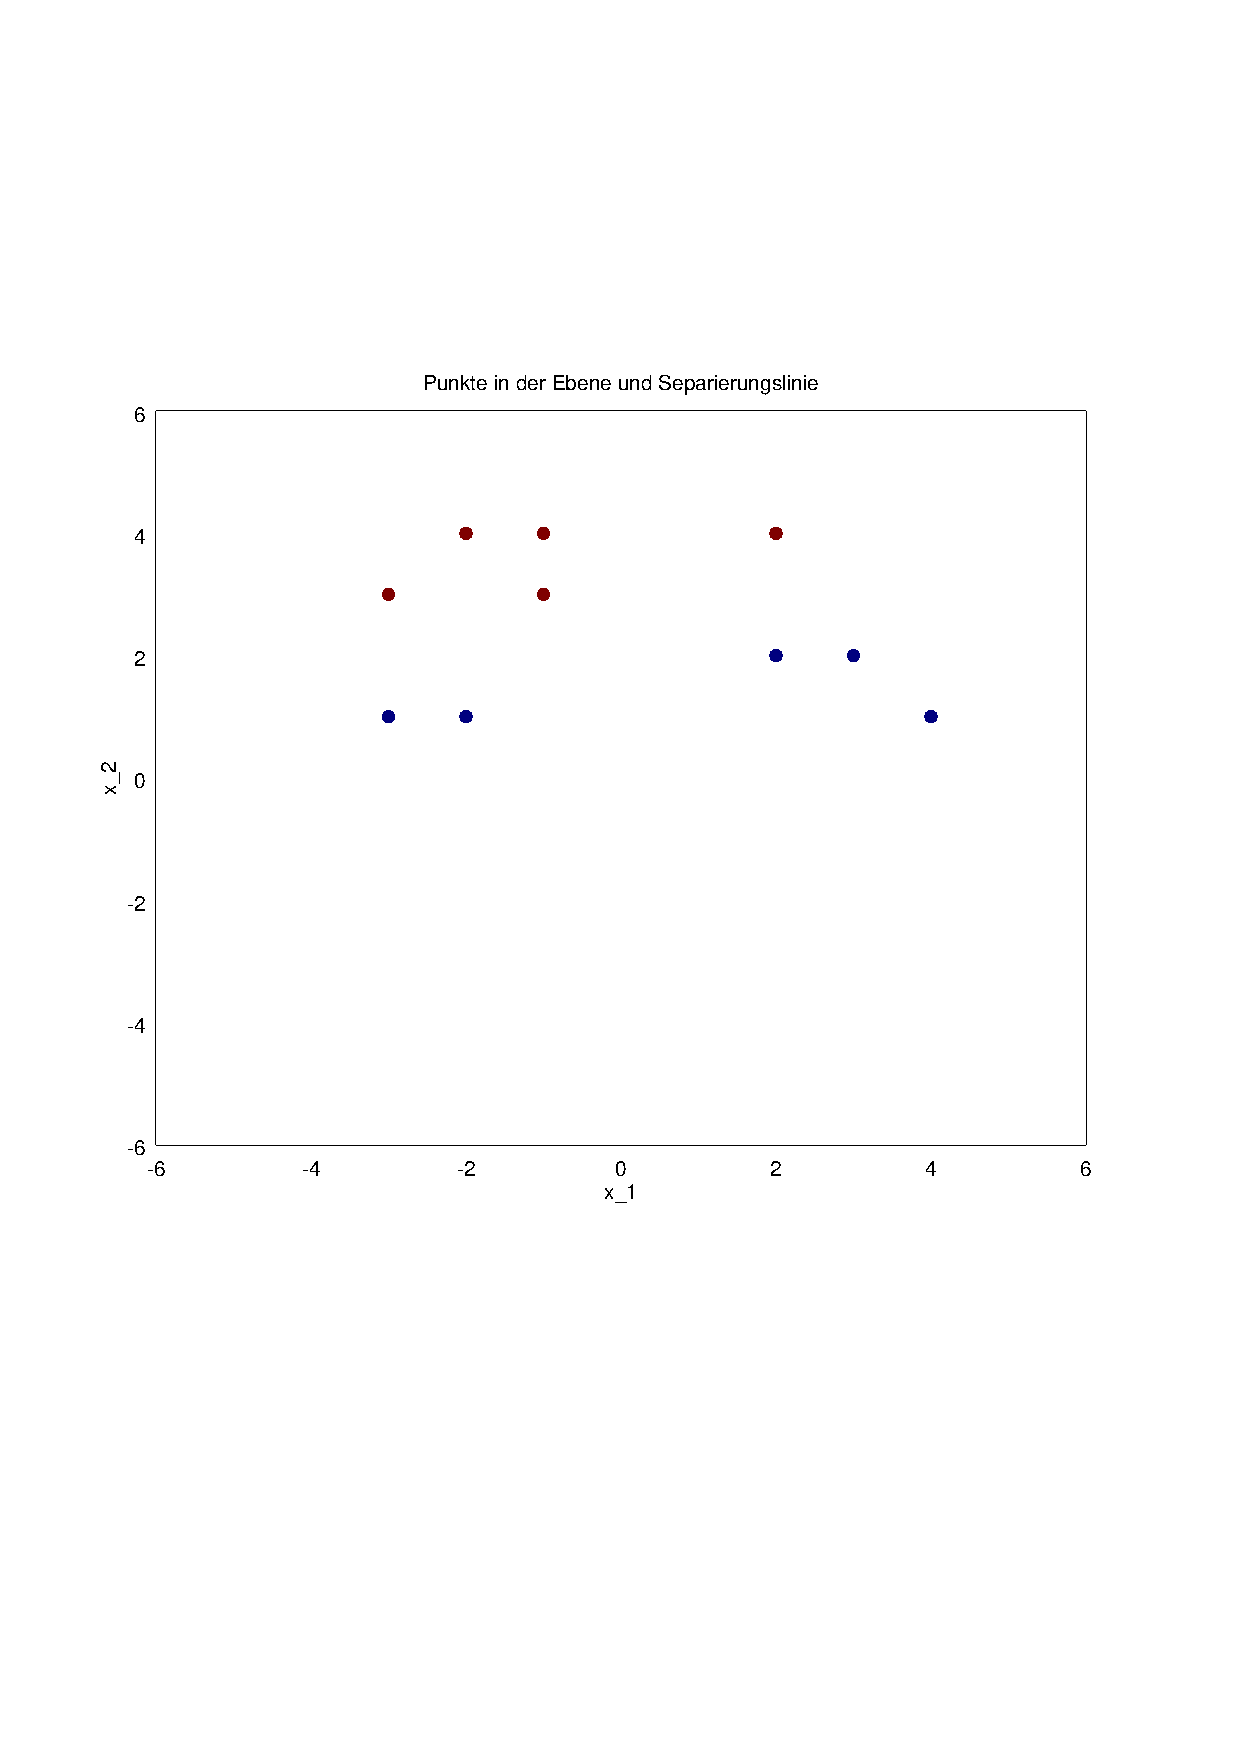
\includegraphics[width=\textwidth]{separated}
        \caption{Separierung nach dem Lernprozess}
    \end{figure}
\end{document}
